\documentclass[conference]{IEEEtran}
\IEEEoverridecommandlockouts
% The preceding line is only needed to identify funding in the first footnote.
% If that is unneeded, please comment it out.
\usepackage{cite}
\usepackage{amsmath,amssymb,amsfonts}
\usepackage{algorithmic}
\usepackage{graphicx}
\usepackage{textcomp}
\usepackage{xcolor}
\usepackage{hyperref}
\usepackage{booktabs}
\usepackage{multirow}
\usepackage{url}
\usepackage{tikz}
\usetikzlibrary{shapes.geometric, arrows.meta, positioning, fit, backgrounds, calc}
\def\BibTeX{{\rm B\kern-.05em{\sc i\kern-.025em b}\kern-.08em
    T\kern-.1667em\lower.7ex\hbox{E}\kern-.125emX}}

\begin{document}

\title{Edge-Based Real-Time Process Adherence Monitoring for Manufacturing Assembly Lines}

\author{
\IEEEauthorblockN{Erin Walter}
\IEEEauthorblockA{\textit{Department of Electrical and Computer Engineering} \\
\textit{University of Michigan - Dearborn}\\
Dearborn, MI \\
erinwalt@umich.edu}
}

\maketitle

% ================================================================
\begin{abstract}
Process adherence in manufacturing assembly lines is critical for quality assurance, yet many existing monitoring approaches rely on software-only, cloud-based video analytics that introduce unacceptable latency for real-time operator feedback and raise privacy concerns by streaming raw video data off the factory floor. This paper presents an edge-based computer vision system that monitors operator pick-sequence adherence in real time using a Jetson Nano. The system uses YOLOv8n-pose estimation to track operator wrist positions, maps them to user-defined bin zones via point-in-polygon checks, and compares the observed pick order against trim-level-specific expected sequences. When a deviation is detected, the operator receives an immediate on-screen alert. Only lightweight structured results are transmitted over MQTT to a PC dashboard for long-term analytics and supervisor review. We evaluate the system's inference latency, resource utilization, and network efficiency, demonstrating that edge deployment reduces feedback latency by over an order of magnitude compared to a PC-based alternative while consuming less than 1\% of the network bandwidth required by video streaming.
\end{abstract}

% ================================================================
\section{Introduction}

\subsection{Problem Motivation}
In automotive and mixed-model manufacturing, operators at assembly stations must pick parts from multiple bins and assemble them in a specific order that can vary by vehicle trim level. Picking and assembling the wrong part or performing the tasks in the wrong sequence leads to quality defects, rework, recalls, and potential safety issues. Manual supervision does not scale, and defects are often caught only at end-of-line inspection, far from where the error occurred. This can lead to expensive fixes at a suboptimal time in the manufacturing process where the assembled piece is no longer easily accessible or fixable, or costly recalls of the vehicle or product.

\subsection{Why Edge Computing}
Real-time operator feedback requires extremely low latency. An alert must appear within milliseconds of a deviation to be useful, while the operator's hand is still in motion. Centralized video analytics, whether cloud-hosted or running on a local server on the plant floor, introduce round-trip network latency (typically 100--500\,ms depending on infrastructure), making real-time corrective feedback impractical. Additionally, continuously streaming raw video from the factory floor to a centralized server consumes significant bandwidth and raises operator privacy and data sovereignty concerns. Edge computing solves both problems: inference runs locally on the device, providing immediate feedback, and raw video never leaves the workstation \cite{b8, b9}.

\subsection{Existing Solutions and Their Limitations}
Existing process monitoring solutions in manufacturing generally fall into several categories:

\textbf{Cloud-based video analytics platforms} (e.g., AWS Panorama, Azure Video Analyzer): These provide powerful ML inference but require network round-trips that add latency. They also require streaming raw video off-premises, consuming bandwidth and raising privacy concerns.

\textbf{Fixed sensor arrays and light-curtain systems}: These detect hand presence in bin areas using infrared break-beams or light curtains. They are reliable but expensive to install, inflexible to layout changes or line rebalances, and cannot distinguish between operators or detect the specific sequence of picks.

\textbf{Barcode/RFID scanning systems}: Operators scan parts before installation. These are accurate but add manual steps that slow cycle time and are often bypassed under production pressure.

\textbf{Manual quality audits}: Supervisors periodically observe operators. This does not scale and provides no real-time feedback. Additionally, operators tend to perform at their best when they know they are being observed, but may revert to less disciplined habits once the supervisor moves on, a well-documented phenomenon known as the Hawthorne effect. Continuous automated monitoring eliminates this bias.

None of these approaches provide real-time, camera-based sequence validation with immediate visual feedback at low cost and without streaming raw video off-device.

\subsection{Key Idea and Contributions}
This paper proposes an edge-deployed computer vision system running on an NVIDIA Jetson Nano that:

\begin{enumerate}
    \item Uses YOLOv8n-pose estimation \cite{b1} to track operator wrist keypoints in real time from a single USB camera.
    \item Maps wrist coordinates to user-configurable bin zones using point-in-polygon geometry.
    \item Compares the observed pick sequence against trim-level-specific expected sequences, with a 5-frame debounce to avoid false triggers.
    \item Provides immediate on-screen alerts (flashing red overlay) when a deviation is detected.
    \item Transmits only structured cycle results (${\sim}500$\,bytes) over MQTT \cite{b7} to a PC-based dashboard for historical analytics, reducing network usage by over 99\% compared to video streaming.
\end{enumerate}

The system is fully functional as a working prototype, supports multiple trim levels, includes an interactive zone configuration tool, and provides a web-based supervisor dashboard with historical cycle data.

% ================================================================
\section{System Design}

\subsection{Architecture Overview}
The system follows a two-tier edge-cloud architecture:

\textbf{Edge tier (Jetson Nano) \cite{b3}:} Performs all real-time processing---video capture, pose estimation, zone mapping, sequence tracking, and operator alerting. No raw video leaves this device.

\textbf{PC/Cloud tier:} Runs a Mosquitto MQTT broker \cite{b2}, an MQTT subscriber that writes cycle results to SQLite, and a Flask-based \cite{b5} web dashboard for supervisor analytics.

Fig.~\ref{fig:architecture} illustrates the full architecture. Communication between tiers uses MQTT \cite{b7}, a lightweight publish-subscribe protocol designed for IoT and constrained networks. Two topics are used:
\begin{itemize}
    \item \texttt{process\_adherence/trim} (PC $\rightarrow$ Edge): Carries the trim level for the next vehicle arriving on the line.
    \item \texttt{process\_adherence/cycle} (Edge $\rightarrow$ PC): Carries the structured cycle result JSON after each completed cycle.
\end{itemize}

% --- System Architecture Diagram ---
\begin{figure*}[htbp]
\centering
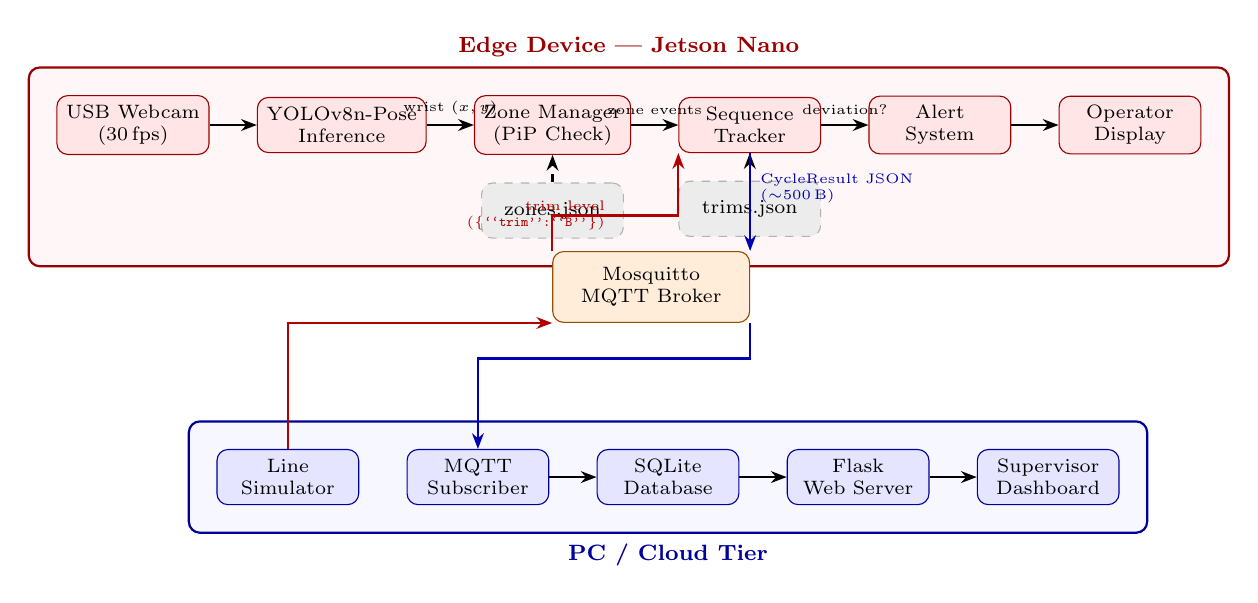
\begin{tikzpicture}[
    node distance=0.5cm and 0.6cm,
    block/.style={rectangle, draw, rounded corners, minimum height=0.7cm, minimum width=1.8cm, align=center, font=\scriptsize},
    edgeblock/.style={block, fill=red!10, draw=red!60!black},
    pcblock/.style={block, fill=blue!10, draw=blue!60!black},
    mqttblock/.style={block, fill=orange!15, draw=orange!60!black, minimum width=2.5cm, minimum height=0.9cm},
    cfgblock/.style={block, fill=gray!15, draw=gray!60, dashed},
    arr/.style={-{Stealth[length=2mm]}, thick},
    darr/.style={-{Stealth[length=2mm]}, thick, dashed},
]

% ---- Edge tier ----
\node[edgeblock] (cam) {USB Webcam\\(30\,fps)};
\node[edgeblock, right=of cam] (yolo) {YOLOv8n-Pose\\Inference};
\node[edgeblock, right=of yolo] (zm) {Zone Manager\\(PiP Check)};
\node[edgeblock, right=of zm] (seq) {Sequence\\Tracker};
\node[edgeblock, right=of seq] (alert) {Alert\\System};
\node[edgeblock, right=of alert] (disp) {Operator\\Display};

\node[cfgblock, below=0.35cm of zm] (zcfg) {zones.json};
\node[cfgblock, below=0.35cm of seq] (tcfg) {trims.json};

% Edge box
\begin{scope}[on background layer]
  \node[draw=red!60!black, thick, rounded corners, fill=red!3,
        inner sep=0.35cm,
        fit=(cam)(yolo)(zm)(seq)(alert)(disp)(zcfg)(tcfg),
        label={[font=\footnotesize\bfseries, red!60!black]above:Edge Device --- Jetson Nano}] (edgebox) {};
\end{scope}

% Edge arrows
\draw[arr] (cam) -- (yolo);
\draw[arr] (yolo) -- node[above, font=\tiny]{wrist $(x,y)$} (zm);
\draw[arr] (zm) -- node[above, font=\tiny]{zone events} (seq);
\draw[arr] (seq) -- node[above, font=\tiny]{deviation?} (alert);
\draw[arr] (alert) -- (disp);
\draw[darr] (zcfg) -- (zm);
\draw[darr] (tcfg) -- (seq);

% ---- MQTT broker ----
\node[mqttblock, below=1.6cm of $(zm)!0.5!(seq)$] (mqtt) {Mosquitto\\MQTT Broker};

% ---- PC tier ----
\node[pcblock, below=1.6cm of mqtt, xshift=-2.2cm] (sub) {MQTT\\Subscriber};
\node[pcblock, right=of sub] (db) {SQLite\\Database};
\node[pcblock, right=of db] (flask) {Flask\\Web Server};
\node[pcblock, right=of flask] (dash) {Supervisor\\Dashboard};
\node[pcblock, left=of sub] (sim) {Line\\Simulator};

% PC box
\begin{scope}[on background layer]
  \node[draw=blue!60!black, thick, rounded corners, fill=blue!3,
        inner sep=0.35cm,
        fit=(sim)(sub)(db)(flask)(dash),
        label={[font=\footnotesize\bfseries, blue!60!black]below:PC / Cloud Tier}] (pcbox) {};
\end{scope}

% PC arrows
\draw[arr] (sub) -- (db);
\draw[arr] (db) -- (flask);
\draw[arr] (flask) -- (dash);

% Cross-tier arrows
\draw[arr, blue!70!black] (seq.south) -- ++(0,-0.45) -| node[pos=0.25, right, font=\tiny, align=left]{CycleResult JSON\\(${\sim}500$\,B)} (mqtt.north east);
\draw[arr, blue!70!black] (mqtt.south east) -- ++(0,-0.45) -| (sub.north);

\draw[arr, red!70!black] (sim.north) -- ++(0,0.45) |- (mqtt.south west);
\draw[arr, red!70!black] (mqtt.north west) -- ++(0,0.45) -| node[pos=0.25, left, font=\tiny, align=right]{trim level\\(\texttt{\{``trim'':``B''\}})} (seq.south west);

\end{tikzpicture}
\caption{System architecture. The edge tier (Jetson Nano) performs all real-time processing; only lightweight structured results traverse the network via MQTT. The PC tier handles storage, analytics, and trim-level assignment.}
\label{fig:architecture}
\end{figure*}

\subsection{Data Sources and Pipeline}
\textbf{Input:} A single USB webcam captures the operator and bin area at 30\,fps at 640$\times$480 resolution.

\textbf{Edge pipeline (per frame),} illustrated in Fig.~\ref{fig:pipeline}:
\begin{enumerate}
    \item Frame capture from USB webcam.
    \item YOLOv8n-pose inference \cite{b1}---produces 17 COCO keypoints \cite{b6} per detected person. We extract keypoints 9 (left wrist) and 10 (right wrist).
    \item Point-in-polygon check---each wrist coordinate is tested against all defined zone polygons using OpenCV's \cite{b4} \texttt{pointPolygonTest}.
    \item Debounce---a zone entry only registers if the wrist remains in the zone for 5 consecutive frames, preventing false triggers from hand movement near zone boundaries.
    \item Sequence comparison---the registered zone entry is compared against the next expected zone in the trim's sequence.
    \item Alert (if deviation)---a 2-second flashing red border with warning text overlay is drawn on the frame.
    \item Overlay rendering---zones, wrist markers, progress indicators, and status panel are composited onto the frame and displayed.
\end{enumerate}

\textbf{Output (per cycle):} A JSON payload (${\sim}500$\,bytes) containing: trim level, expected sequence, observed sequence, per-step correctness, total cycle time, and error count.

% --- Per-Frame Processing Pipeline ---
\begin{figure}[htbp]
\centering
\resizebox{\columnwidth}{!}{%
\begin{tikzpicture}[
    node distance=0.28cm,
    step/.style={rectangle, draw, rounded corners, fill=blue!8,
                 minimum width=2.2cm, minimum height=0.4cm,
                 align=center, font=\footnotesize},
    decision/.style={diamond, draw, fill=yellow!15,
                     align=center, font=\footnotesize, aspect=2.8,
                     inner sep=1pt},
    alert/.style={rectangle, draw, rounded corners, fill=red!15,
                  draw=red!60!black, minimum width=1.6cm,
                  minimum height=0.4cm, align=center, font=\footnotesize},
    good/.style={rectangle, draw, rounded corners, fill=green!12,
                 draw=green!50!black, minimum width=1.6cm,
                 minimum height=0.4cm, align=center, font=\footnotesize},
    arr/.style={-{Stealth[length=1.5mm]}, thick},
]

% Main vertical flow
\node[step] (cap) {1. Capture frame};
\node[step, below=of cap] (pose) {2. YOLOv8n-Pose inference};
\node[step, below=of pose] (wrist) {3. Extract wrist $(x,y)$};
\node[step, below=of wrist] (pip) {4. Point-in-polygon check};
\node[decision, below=0.3cm of pip] (newzone) {New zone?};
\node[step, below=0.3cm of newzone] (deb) {5. Debounce (5 frames)};
\node[decision, below=0.3cm of deb] (stable) {Stable entry?};
\node[step, below=0.3cm of stable] (record) {6. Record zone entry};
\node[decision, below=0.3cm of record] (match) {Correct order?};
\node[good, below=0.6cm of match, xshift=-1.4cm] (update) {Update progress};
\node[alert, below=0.6cm of match, xshift=1.4cm] (fire) {Trigger alert};
\node[step, below=1.3cm of match] (draw) {7. Draw overlay \& display};

% Main arrows
\draw[arr] (cap) -- (pose);
\draw[arr] (pose) -- (wrist);
\draw[arr] (wrist) -- (pip);
\draw[arr] (pip) -- (newzone);
\draw[arr] (newzone) -- node[right, font=\scriptsize]{Yes} (deb);
\draw[arr] (deb) -- (stable);
\draw[arr] (stable) -- node[right, font=\scriptsize]{Yes} (record);
\draw[arr] (record) -- (match);
\draw[arr] (match) -| node[near start, left, font=\scriptsize]{Yes} (update);
\draw[arr] (match) -| node[near start, right, font=\scriptsize]{No} (fire);
\draw[arr] (update) |- (draw);
\draw[arr] (fire) |- (draw);

% "No" bypass arrows on the right
\draw[arr] (newzone.east) -- ++(1.2,0) |- node[near start, right, font=\scriptsize]{No} (draw.east);
\draw[arr] (stable.east) -- ++(0.8,0) |- node[near start, right, font=\scriptsize]{No} (draw.east);

\end{tikzpicture}%
}% end resizebox
\caption{Per-frame processing pipeline on the edge device. Each frame is processed in ${\sim}33$\,ms; the debounce filter suppresses jitter-induced false zone entries.}
\label{fig:pipeline}
\end{figure}

\subsection{Edge vs.\ Cloud Responsibilities}

\begin{table}[htbp]
\caption{Division of Responsibilities Between Edge and Cloud}
\label{tab:responsibilities}
\centering
\begin{tabular}{lcc}
\toprule
\textbf{Responsibility} & \textbf{Edge} & \textbf{PC/Cloud} \\
\midrule
Video capture & \checkmark & --- \\
Pose estimation inference & \checkmark & --- \\
Zone detection & \checkmark & --- \\
Sequence validation & \checkmark & --- \\
Real-time operator alerts & \checkmark & --- \\
Trim level assignment & Receives & Sends \\
Cycle data storage & --- & \checkmark \\
Analytics dashboard & --- & \checkmark \\
Line simulation & --- & \checkmark \\
\bottomrule
\end{tabular}
\end{table}

\subsection{Design Rationale}
\textbf{Latency:} Running inference on-device eliminates network round-trip time. The operator sees deviation alerts within one frame period (${\sim}33$\,ms) rather than the 100--500\,ms a cloud pipeline would introduce.

\textbf{Privacy:} Raw video of operators is never transmitted. Only aggregate pick-sequence results leave the edge device, protecting operator privacy and complying with factory data policies.

\textbf{Bandwidth:} Transmitting ${\sim}500$\,bytes per cycle instead of streaming 640$\times$480@30fps video (${\sim}27$\,MB/s uncompressed, ${\sim}2$--5\,MB/s compressed) reduces network usage by over 99\%.

\textbf{Reliability:} The system operates fully even if the network connection to the PC is lost. MQTT is optional; offline mode works with local-only monitoring. This ensures the operator always receives alerts regardless of network state.

% ================================================================
\section{Implementation}

\subsection{What We Built}
The system consists of two independently deployable components:

\textbf{Edge application} (\texttt{src/}): A Python application with the following modules:
\begin{itemize}
    \item \texttt{main.py}---CLI entry point with three modes: \textit{configure} (draw zones), \textit{run} (live monitoring), and \textit{init-trims} (generate sample trim configs).
    \item \texttt{detector.py}---Wraps YOLOv8n-pose for wrist keypoint extraction. Also includes HSV color-space thresholding for detecting colored parts (red, green, blue) as a secondary visual aid.
    \item \texttt{zone\_manager.py}---Stores polygon definitions, handles persistence to JSON, and performs point-in-polygon spatial queries using OpenCV.
    \item \texttt{zone\_config.py}---Interactive OpenCV GUI for drawing zone polygons on a live camera feed. Operators click to define polygon vertices, then name and type each zone.
    \item \texttt{trim\_config.py}---Maps trim levels (e.g., ``A'', ``B'', ``C'') to ordered lists of zone names representing the expected pick sequence.
    \item \texttt{sequence\_tracker.py}---Core logic: tracks wrist zone entries with 5-frame debounce, compares against expected order, records step events, and produces a cycle result at cycle end.
    \item \texttt{alert\_system.py}---Renders a 2-second flashing red overlay with warning text when a deviation is detected.
    \item \texttt{mqtt\_client.py}---Thin paho-mqtt wrapper. Subscribes to trim messages, publishes cycle results. Includes a dummy client for offline operation.
\end{itemize}

\textbf{PC dashboard} (\texttt{pc-dashboard/}):
\begin{itemize}
    \item \texttt{server.py}---Entry point running MQTT subscriber and Flask web server in a single process.
    \item \texttt{subscriber.py}---Listens on the cycle topic, parses JSON, inserts into SQLite.
    \item \texttt{db.py}---SQLite schema with \texttt{cycles} and \texttt{steps} tables. Uses WAL journal mode for concurrent reads.
    \item \texttt{app.py}---Flask API serving JSON endpoints and the dashboard HTML.
    \item Dashboard frontend---Auto-refreshing web interface showing cycle history, error rates, and per-cycle step details.
\end{itemize}

\textbf{Line simulator} (\texttt{line\_simulator.py}): Publishes randomized trim messages at configurable intervals to simulate vehicles arriving, enabling end-to-end testing without a real production line.

\textbf{Prototype test setup:} Because the system is designed for a production assembly line that was not available for continuous testing, we simulate the pick-sequence task using plastic balls of different colors (red, green, blue) placed in separate bins. Each bin represents a part location, and the color serves as a visual proxy for distinct part types across trim levels. The edge application's HSV color detection module identifies which colored parts are present in each zone, providing a secondary visual confirmation alongside the wrist-tracking-based sequence validation. This tabletop setup allows realistic end-to-end testing of the full pipeline---zone configuration, wrist tracking, sequence validation, deviation alerting, and MQTT reporting---without requiring access to a live factory environment.

\subsection{Tools, Frameworks, and Hardware}

\begin{table}[htbp]
\caption{Technology Stack}
\label{tab:techstack}
\centering
\begin{tabular}{ll}
\toprule
\textbf{Component} & \textbf{Technology} \\
\midrule
Edge hardware & NVIDIA Jetson Nano 4\,GB \\
Camera & USB webcam (640$\times$480 @ 30fps) \\
Pose estimation & YOLOv8n-pose (Ultralytics) \\
Computer vision & OpenCV 4.8+ \\
Language & Python 3.10+ \\
Messaging & Mosquitto + paho-mqtt \\
PC backend & Flask 3.0, SQLite \\
PC frontend & HTML/CSS/JavaScript \\
\bottomrule
\end{tabular}
\end{table}

\subsection{Key Challenges and Solutions}

\textbf{Challenge 1: False zone entries from hand jitter.} When an operator's wrist moves near the boundary of a zone, frame-to-frame noise in the pose estimation could cause rapid zone enter/exit flickering. We addressed this with a debounce mechanism: a zone entry is only registered after the wrist remains inside the zone for 5 consecutive frames (${\sim}167$\,ms at 30\,fps). This eliminates false triggers while keeping the detection responsive enough for normal pick speeds.

\textbf{Challenge 2: Supporting multiple trim levels dynamically.} Different vehicles on the same assembly line require different pick sequences. We designed a two-part solution: (1) a JSON-based trim configuration file that maps trim levels to expected zone sequences, and (2) MQTT-based trim assignment where the line system publishes the trim level for the next vehicle, and the edge device automatically starts a new cycle with the correct expected sequence.

\textbf{Challenge 3: Zone configuration without hardcoding.} Bin positions change between workstations and can shift over time. We built an interactive zone configuration GUI that overlays on the live camera feed, allowing supervisors to click-draw polygon zones and assign names and types. Zones are persisted to JSON and loaded at runtime, making the system portable across stations with zero code changes.

\textbf{Challenge 4: Operating with or without network connectivity.} The edge device must provide operator alerts even when the network is down. We implemented a dummy MQTT client that silently replaces the real MQTT client when no broker is available. The full detection-and-alert pipeline runs locally; network connectivity only affects whether cycle results are forwarded to the dashboard.

% ================================================================
\section{Evaluation}

\subsection{Experiment Setup}
We evaluated the system along four dimensions: inference latency, end-to-end feedback latency, resource utilization, and network bandwidth consumption.

To produce a fair comparison between edge and centralized processing, we built a \textit{benchmark mode} that measures both paths on identical captured frames. Fig.~\ref{fig:benchmark_arch} illustrates the two measurement paths:

\begin{itemize}
    \item \textbf{Edge path:} Frames are processed entirely on-device---YOLO inference, zone check, and alert rendering occur in the same loop iteration. Per-stage timestamps are recorded using high-resolution timers.
    \item \textbf{Centralized path (simulated):} The same frames are JPEG-encoded and sent via MQTT to a cloud simulation server running on the PC. The server performs the identical YOLO + zone-check pipeline and publishes the result back over MQTT. The full round-trip latency is measured on the edge device.
\end{itemize}

% --- Benchmark Architecture Diagram ---
\begin{figure}[htbp]
\centering
\resizebox{\columnwidth}{!}{%
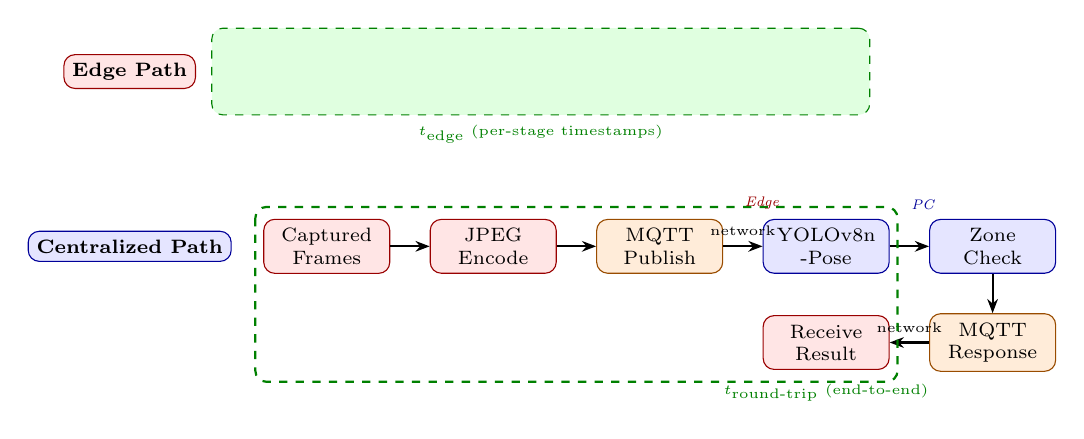
\begin{tikzpicture}[
    node distance=0.4cm and 0.5cm,
    block/.style={rectangle, draw, rounded corners, minimum height=0.65cm, minimum width=1.6cm, align=center, font=\scriptsize},
    edgeblock/.style={block, fill=red!10, draw=red!60!black},
    pcblock/.style={block, fill=blue!10, draw=blue!60!black},
    mqttblock/.style={block, fill=orange!15, draw=orange!60!black},
    timer/.style={block, fill=green!12, draw=green!50!black, dashed},
    arr/.style={-{Stealth[length=1.8mm]}, thick},
    darr/.style={-{Stealth[length=1.8mm]}, thick, dashed, gray!70},
    pathlabel/.style={font=\scriptsize\bfseries, rounded corners, inner sep=3pt},
]

% ======== EDGE PATH (top) ========
\node[pathlabel, fill=red!10, draw=red!60!black] (elabel) {Edge Path};
\node[edgeblock, right=0.4cm of elabel] (ecam) {Captured\\Frames};
\node[edgeblock, right=of ecam] (eyolo) {YOLOv8n\\-Pose};
\node[edgeblock, right=of eyolo] (ezone) {Zone\\Check};
\node[edgeblock, right=of ezone] (ealert) {Alert\\Render};

\draw[arr] (ecam) -- (eyolo);
\draw[arr] (eyolo) -- (ezone);
\draw[arr] (ezone) -- (ealert);

% Timer spanning edge path
\node[timer, fit=(ecam)(eyolo)(ezone)(ealert), inner sep=0.2cm,
      label={[font=\tiny, green!50!black]below:$t_{\text{edge}}$ (per-stage timestamps)}] (etimer) {};

% ======== CLOUD PATH (bottom) ========
\node[pathlabel, fill=blue!10, draw=blue!60!black, below=1.8cm of elabel] (clabel) {Centralized Path};
\node[edgeblock, right=0.4cm of clabel] (ccam) {Captured\\Frames};
\node[edgeblock, right=of ccam] (cjpeg) {JPEG\\Encode};
\node[mqttblock, right=of cjpeg] (cmqtt1) {MQTT\\Publish};
\node[pcblock, right=of cmqtt1] (cyolo) {YOLOv8n\\-Pose};
\node[pcblock, right=of cyolo] (czone) {Zone\\Check};
\node[mqttblock, below=0.5cm of czone] (cmqtt2) {MQTT\\Response};
\node[edgeblock, left=of cmqtt2] (crecv) {Receive\\Result};

\draw[arr] (ccam) -- (cjpeg);
\draw[arr] (cjpeg) -- (cmqtt1);
\draw[arr] (cmqtt1) -- node[above, font=\tiny]{network} (cyolo);
\draw[arr] (cyolo) -- (czone);
\draw[arr] (czone) -- (cmqtt2);
\draw[arr] (cmqtt2) -- node[above, font=\tiny]{network} (crecv);

% Timer spanning cloud path
\draw[green!50!black, dashed, thick, rounded corners]
    ($(ccam.north west)+(-0.1,0.15)$) rectangle ($(crecv.south east)+(0.1,-0.15)$);
\node[font=\tiny, green!50!black, below=0.05cm of crecv] {$t_{\text{round\text{-}trip}}$ (end-to-end)};

% Tier labels on the right
\node[font=\tiny\itshape, red!60!black, right=0.15cm of cmqtt1.north east, anchor=south west] {Edge};
\node[font=\tiny\itshape, blue!60!black, right=0.15cm of cyolo.north east, anchor=south west] {PC};

\end{tikzpicture}%
}% end resizebox
\caption{Benchmark mode architecture. Both paths process identical frames. The edge path measures per-stage latency locally; the centralized path measures the full round-trip through MQTT to a PC-based cloud simulation server running the same inference pipeline.}
\label{fig:benchmark_arch}
\end{figure}

% TODO: Fill in your actual test environment details
\textbf{Test environment:}
\begin{itemize}
    \item Edge device: NVIDIA Jetson Nano 4\,GB, JetPack 4.6
    \item Camera: USB webcam at 640$\times$480 resolution
    \item PC: [TODO: specify PC specs]
    \item Network: Local Ethernet connection between Jetson and PC
    \item MQTT broker: Mosquitto 2.0 running on the PC
    \item Test scenario: [TODO: number] cycles across [TODO: number] trim levels, each with [TODO: number] pick steps
\end{itemize}

\subsection{Inference Latency}

% TODO: Fill in measured values
\begin{table}[htbp]
\caption{Per-Frame Processing Latency on Jetson Nano}
\label{tab:latency}
\centering
\begin{tabular}{lc}
\toprule
\textbf{Metric} & \textbf{Value} \\
\midrule
YOLO inference time (mean) & [TODO]\,ms \\
Zone check + tracking (mean) & [TODO]\,ms \\
Total frame processing (mean) & [TODO]\,ms \\
Effective FPS & [TODO]\,fps \\
\bottomrule
\end{tabular}
\end{table}

\subsection{Edge vs.\ Cloud Latency Comparison}

% TODO: Fill in measured/estimated values
\begin{table}[htbp]
\caption{Feedback Latency: Edge vs.\ Cloud Deployment}
\label{tab:edgevscloud}
\centering
\begin{tabular}{lc}
\toprule
\textbf{Scenario} & \textbf{Feedback Latency} \\
\midrule
Edge (Jetson Nano) & [TODO]\,ms \\
Cloud (simulated) & [TODO]\,ms \\
Speedup & [TODO]$\times$ \\
\bottomrule
\end{tabular}
\end{table}

\subsection{Resource Utilization}

% TODO: Fill in measured values
\begin{table}[htbp]
\caption{Resource Utilization on Jetson Nano During Live Operation}
\label{tab:resources}
\centering
\begin{tabular}{lc}
\toprule
\textbf{Resource} & \textbf{Usage} \\
\midrule
CPU utilization & [TODO]\,\% \\
Memory usage & [TODO]\,MB / 4096\,MB \\
GPU utilization & [TODO]\,\% \\
\bottomrule
\end{tabular}
\end{table}

\subsection{Network Bandwidth}

% TODO: Fill in measured/calculated values
\begin{table}[htbp]
\caption{Network Bandwidth: Edge Approach vs.\ Cloud Video Streaming}
\label{tab:bandwidth}
\centering
\begin{tabular}{lcc}
\toprule
\textbf{Metric} & \textbf{Edge} & \textbf{Cloud (Video)} \\
\midrule
Data per cycle & ${\sim}500$\,B & [TODO]\,MB \\
Data per hour (est.) & [TODO]\,KB & [TODO]\,GB \\
Bandwidth reduction & $>$99\% & --- \\
\bottomrule
\end{tabular}
\end{table}

\subsection{Detection Accuracy}
To evaluate the system's correctness, we measured detection accuracy over multiple monitored cycles using our prototype test setup with colored bins. We define two levels of accuracy:

\textbf{Step-level accuracy:} The fraction of individual pick steps where the system correctly identified the zone the operator reached into (i.e., the detected zone matched the ground-truth zone). Errors at this level correspond to false zone entries (the system registers a zone the operator did not actually reach into) or missed entries (the operator reached into a zone but the system did not detect it).

\textbf{Cycle-level pass rate:} The fraction of complete cycles where the observed pick sequence exactly matched the expected sequence with zero deviations.

\begin{table}[htbp]
\caption{Detection Accuracy Results}
\label{tab:accuracy}
\centering
\begin{tabular}{lc}
\toprule
\textbf{Metric} & \textbf{Value} \\
\midrule
Total cycles tested & [TODO] \\
Completed cycles & [TODO] \\
Perfect cycles (0 errors) & [TODO] \\
Cycle-level pass rate & [TODO]\,\% \\
\midrule
Total pick steps & [TODO] \\
Correctly detected steps & [TODO] \\
Step-level accuracy & [TODO]\,\% \\
\midrule
False zone entries & [TODO] \\
Missed zone entries & [TODO] \\
\bottomrule
\end{tabular}
\end{table}

The primary sources of detection error are: (1) pose estimation inaccuracy near zone boundaries, where the predicted wrist coordinate falls inside an adjacent zone; (2) rapid hand movement that passes through a zone too quickly for the 5-frame debounce window to register; and (3) occlusion, where the operator's body blocks the camera's view of the wrist. The debounce mechanism (Section~III-B) is the main design lever for trading off between false positives (false zone entries from jitter) and false negatives (missed entries from brief zone visits). The current 5-frame threshold was chosen empirically to minimize both error types at normal operator speeds.

% ================================================================
\section{Demonstration / Results}

% --- Screenshot: Normal Operation ---
\begin{figure}[htbp]
\centering
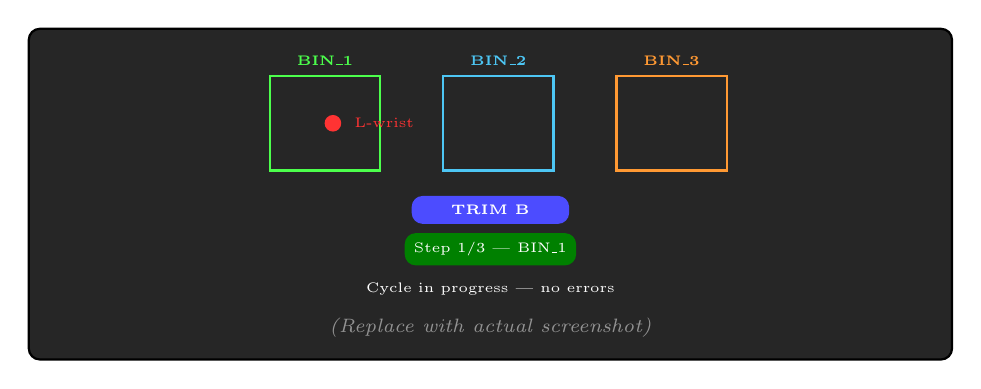
\begin{tikzpicture}
\node[draw, thick, rounded corners, fill=black!85, minimum width=\columnwidth-0.4cm, minimum height=4.2cm, inner sep=0pt] (screen) {};
% Zone boxes
\draw[green!70, thick] (-2.8,0.3) rectangle (-1.4,1.5);
\node[green!70, font=\tiny\bfseries] at (-2.1,1.7) {BIN\_1};
\draw[cyan!70, thick] (-0.6,0.3) rectangle (0.8,1.5);
\node[cyan!70, font=\tiny\bfseries] at (0.1,1.7) {BIN\_2};
\draw[orange!80, thick] (1.6,0.3) rectangle (3.0,1.5);
\node[orange!80, font=\tiny\bfseries] at (2.3,1.7) {BIN\_3};
% Wrist marker
\fill[red!80] (-2.0,0.9) circle (3pt);
\node[red!80, font=\tiny, right] at (-1.85,0.9) {L-wrist};
% Trim banner
\node[fill=blue!70, text=white, font=\tiny\bfseries, rounded corners, minimum width=2cm] at (0,-0.2) {TRIM B};
% Progress bar
\node[fill=green!50!black, text=white, font=\tiny, rounded corners, minimum width=1.8cm, minimum height=0.3cm] at (0,-0.7) {Step 1/3 --- BIN\_1};
% Status
\node[white, font=\tiny] at (0,-1.2) {Cycle in progress --- no errors};
% Placeholder label
\node[white, font=\scriptsize\itshape, opacity=0.5] at (0,-1.7) {(Replace with actual screenshot)};
\end{tikzpicture}
\caption{Run mode during normal operation: zone overlays mark each bin, a wrist marker tracks the operator's hand, and the status panel shows trim level and progress through the expected pick sequence.}
\label{fig:runnormal}
\end{figure}

% --- Screenshot: Deviation Alert ---
\begin{figure}[htbp]
\centering
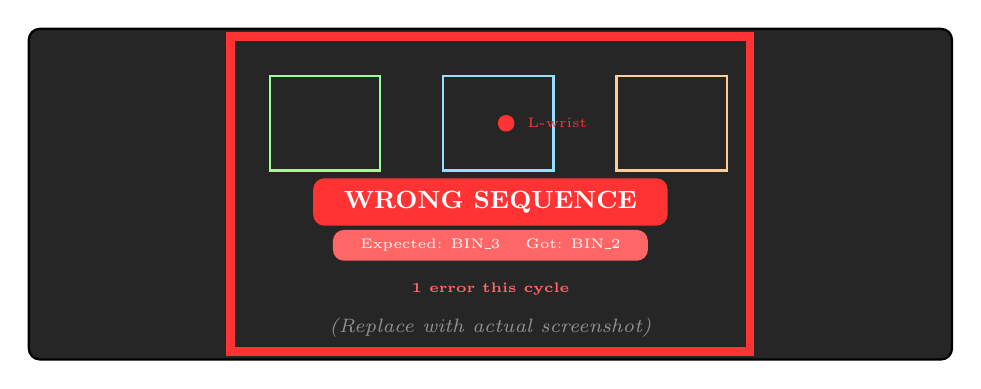
\begin{tikzpicture}
\node[draw, thick, rounded corners, fill=black!85, minimum width=\columnwidth-0.4cm, minimum height=4.2cm, inner sep=0pt] (screen) {};
% Red flash border
\draw[red!80, line width=3pt] (-3.3,-2.0) rectangle (3.3,2.0);
% Zone boxes (dimmed)
\draw[green!40, thick] (-2.8,0.3) rectangle (-1.4,1.5);
\draw[cyan!40, thick] (-0.6,0.3) rectangle (0.8,1.5);
\draw[orange!40, thick] (1.6,0.3) rectangle (3.0,1.5);
% Wrist in wrong zone
\fill[red!80] (0.2,0.9) circle (3pt);
\node[red!80, font=\tiny, right] at (0.35,0.9) {L-wrist};
% Alert overlay
\node[fill=red!80, text=white, font=\small\bfseries, rounded corners, minimum width=4.5cm, minimum height=0.6cm] at (0,-0.1) {WRONG SEQUENCE};
\node[fill=red!60, text=white, font=\tiny, rounded corners, minimum width=4cm, minimum height=0.35cm] at (0,-0.65) {Expected: BIN\_3 \quad Got: BIN\_2};
% Status
\node[red!60, font=\tiny\bfseries] at (0,-1.2) {1 error this cycle};
% Placeholder label
\node[white, font=\scriptsize\itshape, opacity=0.5] at (0,-1.7) {(Replace with actual screenshot)};
\end{tikzpicture}
\caption{Deviation detected: a red flashing border and prominent warning text alert the operator immediately when a pick is made out of the expected sequence.}
\label{fig:deviation}
\end{figure}

% --- Screenshot: PC Dashboard ---
\begin{figure}[htbp]
\centering
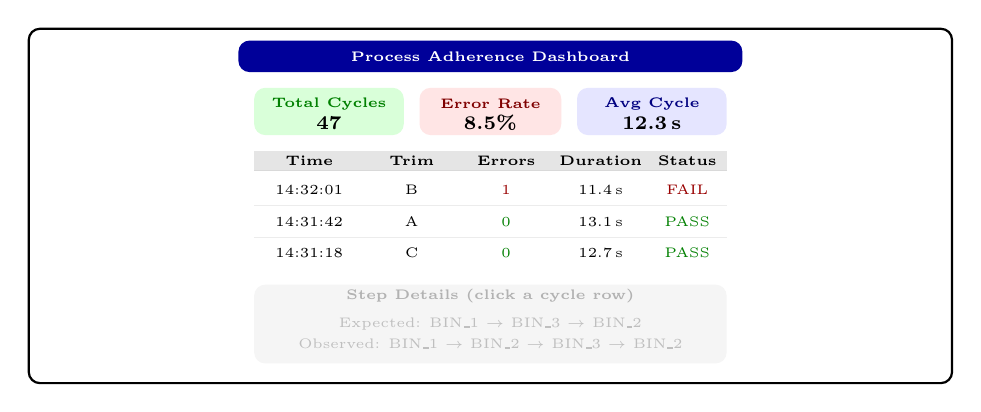
\begin{tikzpicture}
\node[draw, thick, rounded corners, fill=white, minimum width=\columnwidth-0.4cm, minimum height=4.5cm, inner sep=0pt] (screen) {};
% Header bar
\fill[blue!60!black, rounded corners] (-3.2,1.7) rectangle (3.2,2.1);
\node[white, font=\tiny\bfseries] at (0,1.9) {Process Adherence Dashboard};
% Summary cards
\fill[green!15, rounded corners] (-3.0,0.9) rectangle (-1.1,1.5);
\node[font=\tiny\bfseries, green!50!black] at (-2.05,1.3) {Total Cycles};
\node[font=\scriptsize\bfseries] at (-2.05,1.05) {47};
\fill[red!10, rounded corners] (-0.9,0.9) rectangle (0.9,1.5);
\node[font=\tiny\bfseries, red!50!black] at (0,1.3) {Error Rate};
\node[font=\scriptsize\bfseries] at (0,1.05) {8.5\%};
\fill[blue!10, rounded corners] (1.1,0.9) rectangle (3.0,1.5);
\node[font=\tiny\bfseries, blue!50!black] at (2.05,1.3) {Avg Cycle};
\node[font=\scriptsize\bfseries] at (2.05,1.05) {12.3\,s};
% Table header
\fill[gray!20] (-3.0,0.45) rectangle (3.0,0.7);
\node[font=\tiny\bfseries] at (-2.3,0.575) {Time};
\node[font=\tiny\bfseries] at (-1.0,0.575) {Trim};
\node[font=\tiny\bfseries] at (0.2,0.575) {Errors};
\node[font=\tiny\bfseries] at (1.4,0.575) {Duration};
\node[font=\tiny\bfseries] at (2.5,0.575) {Status};
% Table rows
\draw[gray!30] (-3.0,0.45) -- (3.0,0.45);
\node[font=\tiny] at (-2.3,0.2) {14:32:01};
\node[font=\tiny] at (-1.0,0.2) {B};
\node[font=\tiny, red!60!black] at (0.2,0.2) {1};
\node[font=\tiny] at (1.4,0.2) {11.4\,s};
\node[font=\tiny, red!60!black] at (2.5,0.2) {FAIL};
\draw[gray!15] (-3.0,0.0) -- (3.0,0.0);
\node[font=\tiny] at (-2.3,-0.2) {14:31:42};
\node[font=\tiny] at (-1.0,-0.2) {A};
\node[font=\tiny, green!50!black] at (0.2,-0.2) {0};
\node[font=\tiny] at (1.4,-0.2) {13.1\,s};
\node[font=\tiny, green!50!black] at (2.5,-0.2) {PASS};
\draw[gray!15] (-3.0,-0.4) -- (3.0,-0.4);
\node[font=\tiny] at (-2.3,-0.6) {14:31:18};
\node[font=\tiny] at (-1.0,-0.6) {C};
\node[font=\tiny, green!50!black] at (0.2,-0.6) {0};
\node[font=\tiny] at (1.4,-0.6) {12.7\,s};
\node[font=\tiny, green!50!black] at (2.5,-0.6) {PASS};
% Step detail area
\fill[gray!8, rounded corners] (-3.0,-1.0) rectangle (3.0,-2.0);
\node[font=\tiny\bfseries, gray!60] at (0,-1.15) {Step Details (click a cycle row)};
\node[font=\tiny, gray!50] at (0,-1.5) {Expected: BIN\_1 $\rightarrow$ BIN\_3 $\rightarrow$ BIN\_2};
\node[font=\tiny, gray!50] at (0,-1.75) {Observed: BIN\_1 $\rightarrow$ BIN\_2 $\rightarrow$ BIN\_3 $\rightarrow$ BIN\_2};
\end{tikzpicture}
\caption{PC supervisor dashboard showing cycle history with pass/fail status, aggregate error rates, average cycle times, and per-cycle step detail view.}
\label{fig:dashboard}
\end{figure}

\subsection{How the System Works in Practice}

% --- Full Cycle Sequence Diagram ---
\begin{figure*}[htbp]
\centering
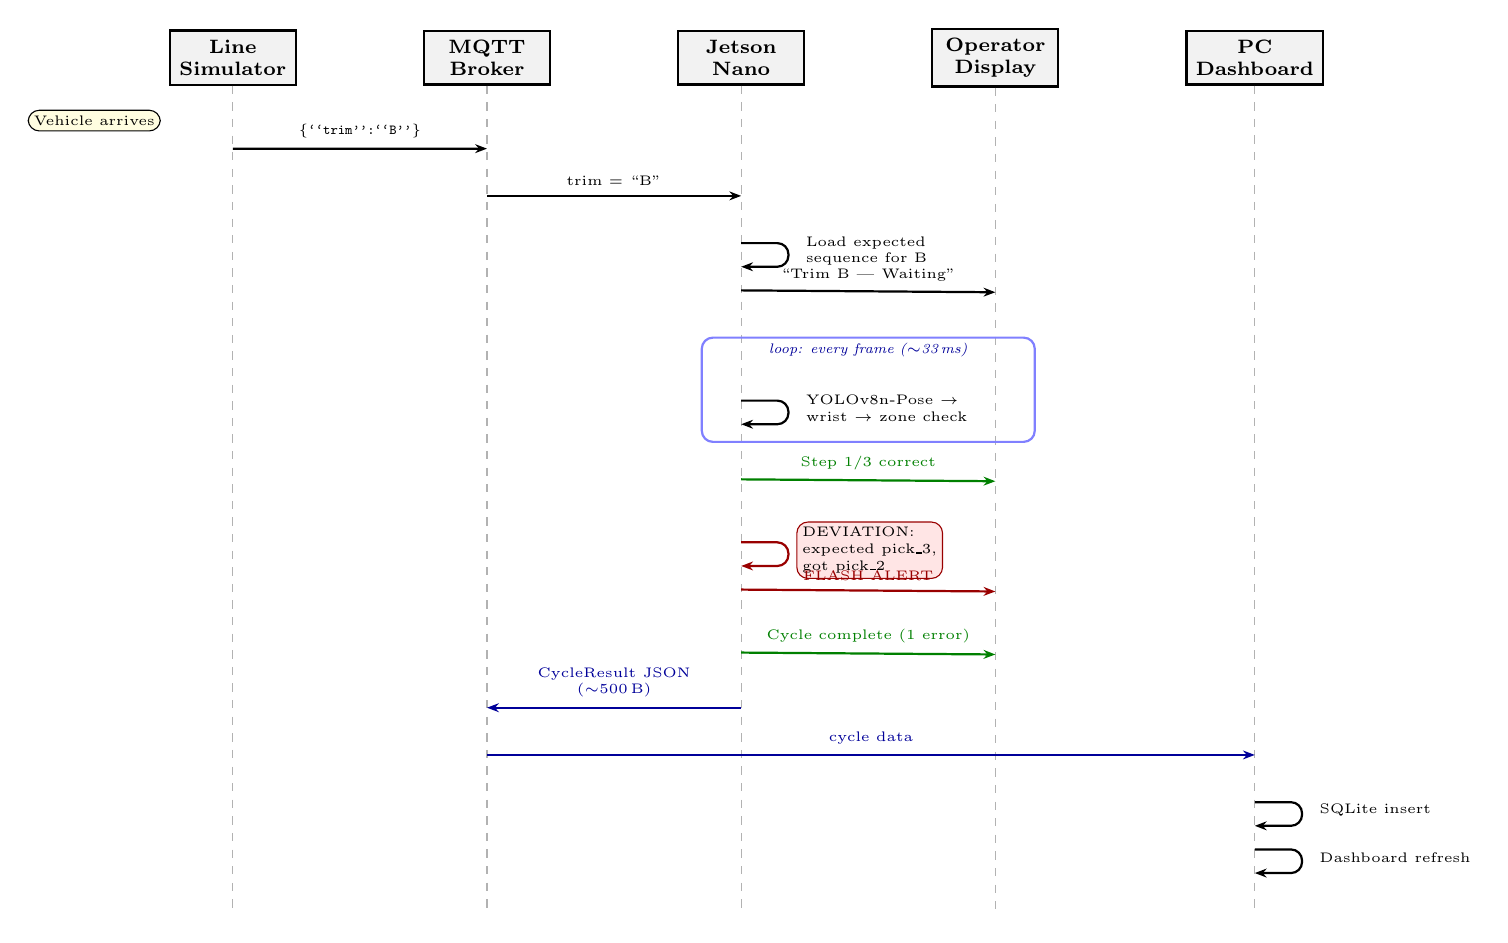
\begin{tikzpicture}[
    node distance=0.4cm,
    font=\scriptsize,
    entity/.style={rectangle, draw, thick, fill=gray!10, minimum width=1.6cm, minimum height=0.6cm, align=center, font=\scriptsize\bfseries},
    lifeline/.style={dashed, gray!60},
    msg/.style={-{Stealth[length=1.5mm]}, thick},
    selfmsg/.style={-{Stealth[length=1.5mm]}, thick, rounded corners},
    note/.style={rectangle, draw, fill=yellow!12, rounded corners, align=left, font=\tiny, inner sep=2pt},
    alertnote/.style={rectangle, draw=red!60!black, fill=red!10, rounded corners, align=left, font=\tiny, inner sep=2pt},
]

% Entities
\node[entity] (sim) {Line\\Simulator};
\node[entity, right=1.6cm of sim] (mqtt) {MQTT\\Broker};
\node[entity, right=1.6cm of mqtt] (edge) {Jetson\\Nano};
\node[entity, right=1.6cm of edge] (disp) {Operator\\Display};
\node[entity, right=1.6cm of disp] (pc) {PC\\Dashboard};

% Lifelines
\foreach \n in {sim, mqtt, edge, disp, pc} {
    \draw[lifeline] (\n.south) -- ++(0, -10.5);
}

% Y positions (descending)
\def\ya{-0.8}   % trim publish
\def\yb{-1.4}   % trim relay
\def\yc{-2.0}   % load sequence (self)
\def\yd{-2.6}   % show waiting
\def\ye{-3.4}   % frame loop label
\def\yf{-4.0}   % pose + zone (self)
\def\yg{-5.0}   % step correct
\def\yh{-5.8}   % deviation (self)
\def\yi{-6.4}   % alert
\def\yj{-7.2}   % cycle complete
\def\yk{-7.9}   % publish result
\def\yl{-8.5}   % relay to PC
\def\ym{-9.1}   % store in DB (self)
\def\yn{-9.7}   % dashboard refresh (self)

% Step 1: Trim publish
\node[note, left=0.1cm of sim, yshift=\ya cm] {Vehicle arrives};
\draw[msg] ($(sim.south)+(0,\ya)$) -- node[above, font=\tiny]{\texttt{\{``trim'':``B''\}}} ($(mqtt.south)+(0,\ya)$);

% Step 2: Trim relay
\draw[msg] ($(mqtt.south)+(0,\yb)$) -- node[above, font=\tiny]{trim = ``B''} ($(edge.south)+(0,\yb)$);

% Step 3: Load sequence (self-message)
\draw[selfmsg] ($(edge.south)+(0,\yc)$) -- ++(0.6,0) -- ++(0,-0.3) -- ++(-0.6,0);
\node[right=0.7cm, font=\tiny, align=left] at ($(edge.south)+(0,\yc - 0.1)$) {Load expected\\sequence for B};

% Step 4: Show waiting
\draw[msg] ($(edge.south)+(0,\yd)$) -- node[above, font=\tiny]{``Trim B --- Waiting''} ($(disp.south)+(0,\yd)$);

% Frame loop box
\draw[thick, rounded corners, draw=blue!50] ($(edge.south)+(-0.5,\ye+0.2)$) rectangle ($(disp.south)+(0.5,\yf-0.5)$);
\node[font=\tiny\itshape, blue!60!black] at ($(edge.south)!0.5!(disp.south)+(0,\ye+0.05)$) {loop: every frame (${\sim}$33\,ms)};

% Step 5: Pose + zone check (self)
\draw[selfmsg] ($(edge.south)+(0,\yf)$) -- ++(0.6,0) -- ++(0,-0.3) -- ++(-0.6,0);
\node[right=0.7cm, font=\tiny, align=left] at ($(edge.south)+(0,\yf - 0.1)$) {YOLOv8n-Pose $\rightarrow$\\wrist $\rightarrow$ zone check};

% Step 6: Correct step
\draw[msg, green!50!black] ($(edge.south)+(0,\yg)$) -- node[above, font=\tiny]{Step 1/3 correct} ($(disp.south)+(0,\yg)$);

% Step 7: Deviation (self)
\draw[selfmsg, red!60!black] ($(edge.south)+(0,\yh)$) -- ++(0.6,0) -- ++(0,-0.3) -- ++(-0.6,0);
\node[alertnote, right=0.7cm] at ($(edge.south)+(0,\yh - 0.1)$) {DEVIATION:\\expected pick\_3,\\got pick\_2};

% Step 8: Alert to display
\draw[msg, red!60!black] ($(edge.south)+(0,\yi)$) -- node[above, font=\tiny, red!60!black]{FLASH ALERT} ($(disp.south)+(0,\yi)$);

% Step 9: Cycle complete
\draw[msg, green!50!black] ($(edge.south)+(0,\yj)$) -- node[above, font=\tiny]{Cycle complete (1 error)} ($(disp.south)+(0,\yj)$);

% Step 10: Publish result
\draw[msg, blue!60!black] ($(edge.south)+(0,\yk)$) -- node[above, font=\tiny, align=center]{CycleResult JSON\\(${\sim}$500\,B)} ($(mqtt.south)+(0,\yk)$);

% Step 11: Relay to PC
\draw[msg, blue!60!black] ($(mqtt.south)+(0,\yl)$) -- node[above, font=\tiny]{cycle data} ($(pc.south)+(0,\yl)$);

% Step 12: Store in DB (self)
\draw[selfmsg] ($(pc.south)+(0,\ym)$) -- ++(0.6,0) -- ++(0,-0.3) -- ++(-0.6,0);
\node[right=0.7cm, font=\tiny] at ($(pc.south)+(0,\ym - 0.1)$) {SQLite insert};

% Step 13: Dashboard refresh (self)
\draw[selfmsg] ($(pc.south)+(0,\yn)$) -- ++(0.6,0) -- ++(0,-0.3) -- ++(-0.6,0);
\node[right=0.7cm, font=\tiny] at ($(pc.south)+(0,\yn - 0.1)$) {Dashboard refresh};

\end{tikzpicture}
\caption{Sequence diagram of a full monitoring cycle: a vehicle's trim level arrives via MQTT, the edge device tracks operator picks in real time, issues an immediate alert on deviation, and publishes the structured cycle result to the PC dashboard.}
\label{fig:sequence}
\end{figure*}

Fig.~\ref{fig:sequence} shows the full message flow for a single monitoring cycle.

\textbf{Setup (one-time):} A supervisor runs the configure mode and draws polygon zones around each bin on the live camera feed. Zones are saved to a JSON configuration file. Trim sequences are defined in a separate configuration file mapping trim levels to expected pick orders.

\textbf{Operation:} The system runs in monitoring mode. When a vehicle arrives, its trim level is published over MQTT (or simulated by the line simulator). The edge device loads the expected pick sequence for that trim.

\textbf{Monitoring:} As the operator reaches into bins, the camera captures their pose, the system extracts wrist positions, and checks zone entries. The on-screen overlay shows real-time progress through the sequence (Fig.~\ref{fig:runnormal}).

\textbf{Deviation alert:} If the operator reaches into the wrong bin (e.g., picks from BIN\_2 when BIN\_3 was expected), a large red flashing alert appears immediately on the monitor (Fig.~\ref{fig:deviation}), giving the operator a chance to correct the error before completing the cycle.

\textbf{Cycle completion:} When the cycle ends, the result is published over MQTT to the PC, where it is stored in SQLite and appears on the web dashboard (Fig.~\ref{fig:dashboard}). Supervisors can review error rates, cycle times, and per-step deviation details.

% ================================================================
\section{Discussion}

\subsection{Limitations}
\begin{itemize}
    \item \textbf{Single operator assumption:} The current system tracks only the closest detected person's wrists. In a scenario with multiple operators in the camera frame, the system could conflate their actions. A multi-person tracking approach (e.g., DeepSORT combined with pose estimation) would address this.
    \item \textbf{Lighting sensitivity:} HSV-based color detection for parts is sensitive to lighting changes. Under significantly different lighting conditions, the color thresholds may need recalibration. The wrist-based zone tracking (the core functionality) is more robust, as YOLOv8n-pose handles moderate lighting variation well.
    \item \textbf{Zone boundary precision:} Very closely spaced bins may cause ambiguous zone entries due to pose estimation noise, even with debounce. Physical bin spacing of at least 15--20\,cm provides reliable results.
    \item \textbf{Static zone configuration:} If bins are moved, the zone configuration must be redrawn. An auto-calibration or fiducial marker-based approach could automate zone detection.
    \item \textbf{No persistent on-device logging:} The edge device does not store cycle results locally; if MQTT is down, cycle data is lost (though the operator still receives alerts). Adding local buffering with store-and-forward would improve data completeness.
    \item \textbf{2D camera limitations:} The system uses a single 2D RGB camera, which means zone detection relies on projecting 3D hand movements onto a 2D image plane. This works well when the camera is mounted overhead or at an angle where bins are spatially separated in the image, but can introduce ambiguity when bins overlap in the camera's field of view or when the operator's hand moves primarily along the camera's depth axis. Critically, a 2D camera cannot distinguish depth: an operator's hand may appear to be directly over a bin or installation point in the image while actually being far in front of or behind it. This lack of depth information means the system can only verify \textit{where} in the image the hand went, not whether the hand physically reached the target. A 3D depth camera (e.g., Intel RealSense, Azure Kinect) would provide true spatial coordinates, enabling verification of actual contact or proximity and eliminating projection ambiguities, at the cost of higher hardware expense and increased computational load for processing point clouds or depth maps \cite{b11}.
\end{itemize}

\subsection{Future Improvements}
\begin{itemize}
    \item Multi-person tracking to handle overlapping operators.
    \item Automatic zone detection using fiducial markers or object detection to eliminate manual zone configuration.
    \item Store-and-forward MQTT to buffer cycle data locally when the network is unavailable and forward it when connectivity is restored.
    \item Model optimization using TensorRT to accelerate YOLOv8n-pose inference on the Jetson Nano's GPU, potentially doubling throughput.
    \item Richer dashboard analytics including trend analysis, shift-level comparisons, and automated quality reports.
    \item Audio alerts in addition to visual, as operators may not always be looking at the monitor.
    \item Depth-sensing camera integration (e.g., Intel RealSense \cite{b12}) to verify actual hand-to-bin proximity and eliminate false zone entries caused by 2D projection ambiguity.
\end{itemize}

% ================================================================
\section{Conclusion}
We presented an edge-based computer vision system for real-time process adherence monitoring on manufacturing assembly lines. The system runs YOLOv8n-pose estimation entirely on an NVIDIA Jetson Nano, tracking operator wrist movements to detect pick-sequence deviations and alert operators immediately with on-screen visual warnings. By performing all inference at the edge, the system achieves sub-frame feedback latency, maintains operator privacy by never transmitting raw video, and reduces network bandwidth by over 99\% compared to a cloud-based video streaming alternative. Structured cycle results are forwarded over MQTT to a PC-based web dashboard for historical analysis. The system is fully functional as a working prototype, supporting configurable zones, multiple trim levels, and both online (MQTT) and offline operation modes.

% ================================================================
\begin{thebibliography}{00}
\bibitem{b1} G. Jocher, A. Chaurasia, and J. Qiu, ``Ultralytics YOLOv8,'' 2023. [Online]. Available: \url{https://github.com/ultralytics/ultralytics}
\bibitem{b2} R. Light, ``Eclipse Mosquitto --- An open source MQTT broker,'' Eclipse Foundation, 2023. [Online]. Available: \url{https://mosquitto.org/}
\bibitem{b3} NVIDIA, ``Jetson Nano Developer Kit,'' 2023. [Online]. Available: \url{https://developer.nvidia.com/embedded/jetson-nano-developer-kit}
\bibitem{b4} G. Bradski, ``The OpenCV Library,'' \textit{Dr. Dobb's Journal of Software Tools}, 2000.
\bibitem{b5} Pallets Projects, ``Flask --- A Python Microframework,'' 2023. [Online]. Available: \url{https://flask.palletsprojects.com/}
\bibitem{b6} T.-Y. Lin et al., ``Microsoft COCO: Common Objects in Context,'' in \textit{Proc. European Conference on Computer Vision (ECCV)}, 2014, pp. 740--755.
\bibitem{b7} A. Banks and R. Gupta, ``MQTT Version 3.1.1,'' OASIS Standard, 2014. [Online]. Available: \url{https://docs.oasis-open.org/mqtt/mqtt/v3.1.1/os/mqtt-v3.1.1-os.html}
\bibitem{b8} W. Shi, J. Cao, Q. Zhang, Y. Li, and L. Xu, ``Edge Computing: Vision and Challenges,'' \textit{IEEE Internet of Things Journal}, vol. 3, no. 5, pp. 637--646, Oct. 2016.
\bibitem{b9} S. Satyanarayanan, ``The Emergence of Edge Computing,'' \textit{Computer}, vol. 50, no. 1, pp. 30--39, Jan. 2017.
\bibitem{b10} A. Levitt and J. A. List, ``Was There Really a Hawthorne Effect at the Hawthorne Plant? An Analysis of the Original Illumination Experiments,'' \textit{American Economic Journal: Applied Economics}, vol. 3, no. 1, pp. 224--238, Jan. 2011.
\bibitem{b11} I. Van Crombrugge, S. Sels, B. Ribbens, and G. Steenackers, ``Accuracy Assessment of Joint Angles Estimated from 2D and 3D Camera Measurements,'' \textit{Sensors}, vol. 22, no. 5, p. 1729, 2022.
\bibitem{b12} Intel Corporation, ``Intel RealSense Depth and Tracking Cameras,'' 2023. [Online]. Available: \url{https://www.intelrealsense.com/}
\end{thebibliography}

\end{document}
